\documentclass[10pt]{article}
\usepackage[utf8]{inputenc}
\usepackage[english]{babel}
\usepackage[font=small,labelfont=bf]{caption}
\usepackage{geometry}
\usepackage[sort&compress, numbers]{natbib}
\usepackage{pxfonts}
\usepackage{graphicx}
\usepackage{setspace}
\usepackage{hyperref}
\usepackage{lineno}

% supplemental tables
\newcommand{\questions}{S1}
\newcommand{\topics}{S2}

% supplemental figures
\newcommand{\individualKnowledgeMapsA}{S1}
\newcommand{\individualKnowledgeMapsB}{S2}
\newcommand{\individualKnowledgeMapsC}{S3}
\newcommand{\individualLearningMapsA}{S4}
\newcommand{\individualLearningMapsB}{S5}

\doublespacing
\linenumbers

\title{Geometric models reveal the hidden structure of conceptual knowledge}

\author{Paxton C. Fitzpatrick and Jeremy R.
Manning\textsuperscript{*}\\Dartmouth
College\\\textsuperscript{*}Corresponding author:
jeremy.r.manning@dartmouth.edu}

\date{}

\begin{document}
\maketitle

\begin{abstract} We develop a mathematical framework, based on natural language
processing models, for tracking and characterizing the acquisition of
conceptual knowledge. Our approach embeds each concept in a high dimensional
representation space, where nearby coordinates reflect similar or related
concepts. We tested our approach using behavioral data collected from a group
of college students. In the experiment, we asked the participants to answer
sets of quiz questions interleaved between watching two course videos from the
Khan Academy platform. We applied our framework to the videos' transcripts, and
to text of the quiz questions, to quantify the content of each moment of video
and each quiz question. We used these embeddings, along with participants' quiz
responses, to track how the learners' knowledge changed after watching each
video. Our findings show how a limited set of quiz questions may be used to
construct rich and meaningful representations of what each learner knows, and
how their knowledge changes over time as they learn.

\textbf{Keywords: education, learning, knowledge, concepts, natural language processing}

\end{abstract}


\section*{Introduction}

Suppose that a teacher had access to a complete ``map'' of everything a student
knew. Defining what such a map might even look like, let alone how it might be
constructed or filled in, is itself a non-trivial problem. But if a teacher
\textit{were} to gain access to such a map, how might that change their ability
to teach the student? Perhaps they might start by checking how well the student
knew the to-be-learned information already, or how much they knew about related
concepts. For some students, they could potentially optimize their teaching
efforts to maximize efficiency by focusing primarily on not-yet-known content.
For other students (or other content areas), it might be more effective to
optimize for direct connections between already-known content and any new
material. Observing how the student's knowledge was changing over time, in
response to their training, could also help to guide the teacher.

Designing and building procedures and tools for mapping out knowledge touches
on deep questions about what it means to learn. For example, how do we acquire
conceptual knowledge? Memorizing course lectures or textbook chapters by rote
can lead to the superficial \textit{appearance} of understanding the underlying
content, but achieving true conceptual understanding seems to require something
deeper and richer. Does conceptual understanding entail connecting newly
acquired information to the scaffolding of one's existing knowledge or
experience~\citep{BlayEtal06,CaraMaho03, ConsEtal16, DeacEtal04, SimoEtal04}?
Or weaving a lecture's atomic elements (e.g., its component words) into a
structured network that describes how those individual elements are related?
Conceptual understanding could also involve building a mental model that
transcends the meanings of those individual atomic elements by reflecting the
deeper meaning underlying the gestalt whole~\citep{Kint70, Macl05, ScotEtal07}.

The difference between ``understanding'' and ``memorizing,'' as framed by the
researchers in education, cognitive psychology, and cognitive
neuroscience~\citep{Kato40, Gall00, ScotEtal07, HallGree08, Macl05} has
profound analogs in the fields of natural language processing and natural
language understanding. For example, considering the raw contents of a document
(e.g., its constituent symbols, letters, and words) might provide some
information about what the document is about, just as memorizing a passage
might be used to answer simple questions about the passage~\citep[e.g., whether
it might contain words related to furniture versus physics;][]{LandDuma97,
BleiEtal03, BleiLaff06}. However, modern natural language processing
models~\citep[e.g.,][]{MikoEtal13a, CerEtal18, BrowEtal20} also attempt to
capture the deeper meaning \textit{underlying} those atomic elements. These
models consider not only the co-occurrences of those elements within and across
documents, but also patterns in how those elements appear across different
scales (e.g., sentences, paragraphs, chapters, etc.), the temporal and
grammatical properties of the elements, and other high-level characteristics of
how they are used~\citep{Mann20, Mann21a}. According to these models, the deep
conceptual meaning of a document may be captured by a feature vector in a
high-dimensional representation space, where nearby vectors reflect
conceptually related documents. A model that succeeds at capturing an analog of
``understanding'' is able to assign nearby feature vectors to two conceptually
related documents, \textit{even when the words contained in those documents
have very little overlap}.

Given these insights, what form might the representation of the sum total of a
person's knowledge take? First, we might require a means of systematically
describing or representing the nearly infinite set of possible things a person
could know. Second, we might want to account for potential associations between
different concepts. For example, the concepts of ``fish'' and ``water'' might
be associated in the sense that fish live in water. Third, knowledge may have a
critical dependency structure, such that knowing about a particular concept
might require first knowing about a set of other concepts. For example,
understanding the concept of a fish swimming in water first requires
understanding what fish and water \textit{are}. Fourth, as we learn, our
``current state of knowledge'' should change accordingly. Learning new concepts
should both update our characterizations of ``what is known'' and should also
unlock any now-satisfied dependencies of that newly learned concept so that
they are ``tagged'' as available for future learning.

Here we develop a framework for modelling how knowledge is acquired during
learning. The central idea is to use text embedding models to define the
coordinate systems of two maps: (a) a \textit{knowledge map} that describes the
extent to which each concept is currently known and (b) a \textit{learning map}
that describes the extent to which each concept could be learned. Each location
on these maps represents a single concept, and the geometries are defined such
that related concepts are located nearby in space. We use this framework to
analyze and interpret behavioral data collected from an experiment that has
participants watch and answer conceptual questions about a series of recorded
course lectures.

Our primary research goal is to advance our understanding of what it means to
acquire deep real-world conceptual knowledge. Traditional laboratory approaches
to studying learning and memory (e.g., list learning studies) often draw little
distinction between memorization and understanding. Instead, these studies
typically focus on whether information is effectively encoded or retrieved,
rather than whether the information is \textit{understood}. Approaches to
studying conceptual learning, such as category learning experiments, can start
to investigate the distinction between memorization and understanding, often by
training participants to distinguish arbitrary or random features in otherwise
meaningless categorized stimuli. However the objective of real-world training,
or learning from life experiences more generally, is often to develop new
knowledge that may be applied in \textit{useful} ways in the future. In this
sense, the gap between modern learning theories and modern pedagogical
approaches and classroom learning strategies is enormous: most of our theories
about \textit{how} people learn are inspired by experimental paradigms and
models that have only peripheral relevance to the kinds of learning that
students and teachers actually seek. To help bridge this gap, our study uses
course materials from real online courses to inform, fit, and test models of
real-world conceptual learning. We also provide a ``proof of concept''
demonstration of how our models might be used to construct ``maps'' of what
students know, and how their knowledge changes with training. In addition to
helping to visualize knowledge (and changes in knowledge), we hope that such
maps might lead to real-world tools for improving how we educate.

\section*{Results}

At its core, our main modeling approach is based around a simple assumption
that we sought to test empirically: all else being equal, knowledge about a
given concept is predictive of knowledge about similar or related concepts.
From a geometric perspective, this assumption implies that knowledge is
fundamentally ``smooth.'' In other words, as one moves through a space
representing someone's knowledge (where similar concepts occupy nearby
coordinates), their ``level of knowledge'' should change relatively gradually
throughout that space. To begin to test this smoothness assumption, we sought
to track our participants' knowledge and how it changed over time in response
to training.

We asked our participants to answer questions from several multiple choice
quizzes and watch two lecture videos from the \textit{Khan Academy} platform
(Fig.~\ref{fig:experiment}). One lecture video, entitled \textit{Four
Fundamental Forces}, was about the four fundamental forces in physics: gravity,
strong and weak interactions, and electromagnetism. The second lecture video,
entitled \textit{Birth of Stars}, provides an overview of our current
understanding of how stars form. We selected both lessons to be (a) accessible
to a broad audience, e.g., by minimizing prerequisite knowledge, (b) largely
independent of each other, e.g., so that the two videos focused on different
material and did not depend on each other, and (c) related to each other, e.g.,
so that both videos contained at least \textit{some} similar or overlapping
content. The two videos we selected are introductory, about different primary
concepts, but also touch on ``physics'' and ``astronomy'' themes. We also wrote
a set of multiple choice quiz questions that would enable us to test
participants' knoweldge about each individual video and about related content
not specifically presented in either video (Tab.~\questions). Participants
answered questions randomly drawn from each content area (lecture 1, lecture 2,
and general physics knowledge) across each of three quizzes. Quiz 1 was
intended to assessed participants' knowledge before training; quiz 2 assessed
knowledge after watching the Four Fundamental Forces video (i.e., lecture 1);
and quiz 3 assessed knowledge after watching the Birth of Stars video (i.e.,
lecture 2).

\begin{figure}[tp]
    \centering
    \includegraphics[width=\textwidth]{figs/experiment}
    
    \caption{\textbf{Experimental paradigm.} Participants alternate between
    answering 13-question multiple choice quizzes and watching two Khan academy
    videos. Each quiz contains a mix of 5 questions about lecture 1, 5
    questions about lecture 2, and 3 general physics knowledge questions. The
    specific questions reflected on each quiz, and the orders of each quiz's
    questions, were randomized across participants.}
    
    \label{fig:experiment}
\end{figure}

We trained a text embedding model using sliding windows of text from the two
videos' transcripts (see \textit{Constructing text embeddings of multiple
videos and questions}). We also used the same model (i.e., trained on the
videos' transcripts) to embed the text of each question in our pool. This
yielded, for each second of each video, and for each question, a single topic
vector-- i.e., a coordinate in a text embedding space
(Fig.~\ref{fig:sliding-windows}). Intuitively, each dimension of the embedding
space corresponds to a ``theme'' or ``topic'' reflected in some part(s) of the
videos (Tab.~\topics), and the coordinates in embedding space denote the blend
of themes reflected by a particular excerpt of text (e.g., from part of a
video's transcript, from a question, etc.).

\begin{figure}[tp]
    \centering
    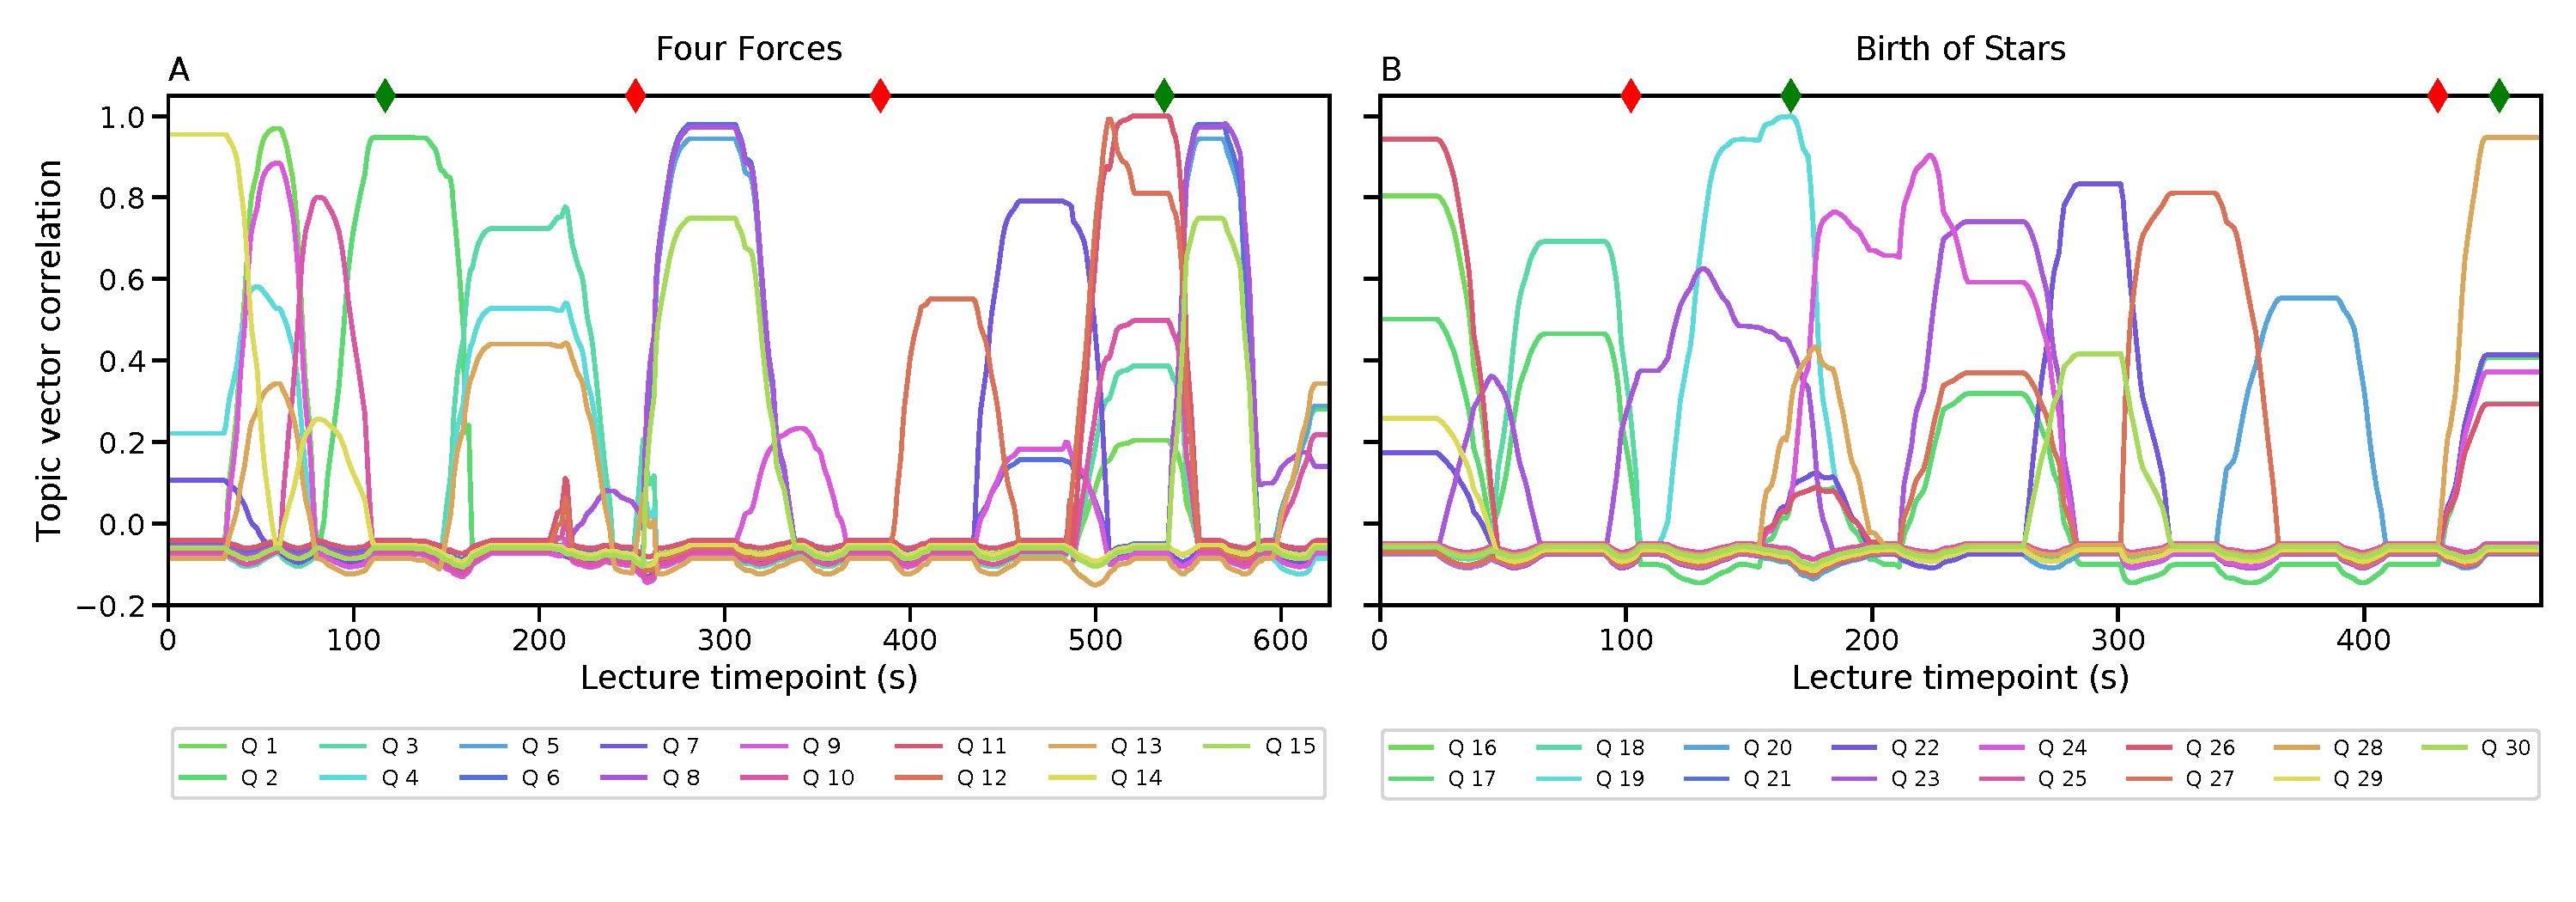
\includegraphics[width=\textwidth]{figs/lecture-question-similarity}
    
    \caption{\textbf{Which parts of each lecture are captured by each
    question?} Each panel displays timeseries plots showing how each question's
    topic vector correlates with each video timepoint's topic vector. The left
    panel displays these correlations for the \textit{Four Fundamental Forces}
    lecture and associated questions, and the right panels displays these
    correlations for the \textit{Birth of Stars} lecture and associated
    questions. The colors denote question identities. The diamonds in each
    panel denote the moment of peak correlation between the indicated
    questions, in the indicated lectures. The associated questions' text, and
    snippets of the lectures' transcripts in the best-matching sliding windows,
    are displayed at the bottom of the figure.}
    
    \label{fig:question-correlations}
\end{figure}

Although a single lecture may be organized a single broad theme at a coarse
scale, at a finer scale each moment of a lecture typically covers a narrower
range of content. We wondered whether a text embedding model trained on the
lectures' transcripts might capture some of this finer scale content. For
example, if a particular question asks about the content from one small part of
a lecture, we wondered whether our text embedding model could be used to
automatically identify the ``matching'' moment(s) in the lecture. When we
correlated each question's topic vector with the topic vectors for each second
of the lectures, we found some evidence that each question is temporally
specific (Fig.~\ref{fig:question-correlations}). In particular, most questions'
topic vectors were maximally correlated with a well-defined range of timepoints
from their corresponding lectures, and the correlations fell off sharply
outside of that range. We also examined the best-matching intervals for each
question qualitatively by comparing the text of the question to the text of the
most-correlated parts of the lectures. Despite that the questions were excluded
from the text embedding model's training set, in general we found a close
correspondence between the conceptual content that each question covered and
the content covered by the best-matching moments of the lectures. Two
representative examples are shown at the bottom of
Fig.~\ref{fig:question-correlations}.

The ability to quantify how much each question is ``asking about'' each moment
of the lectures could enable high-resolution insights into participants'
knowledge. Traditional approaches to estimating how much a student ``knows''
about the content of a given lecture entail computing the proportion of
correctly answered questions. But if two students receive identical scores on
an exam, might our modeling framework help us to gain more naunced insights
into the \textit{specific} content that each student has mastered (or failed to
master)? For example, a student who misses three questions that were all about
the same concept (e.g., concept $A$) will have gotten the same
\textit{proportion} of questions correct as another student who missed three
questions about three \textit{different} concepts (e.g., $A$, $B$, and $C$).
But if we wanted to fill in the ``gaps'' in the two students' understandings,
we might do well to focus on concept $A$ for the first student, but add in
concepts $B$ and $C$ for the second student.

\textbf{JRM STOPPED HERE...}



As a sanity check, we anticipated that our knowledge estimates
should show a content-specific ``boost'' in participants' knowledge after
watching each video.

\begin{figure}[tp]
    \centering
    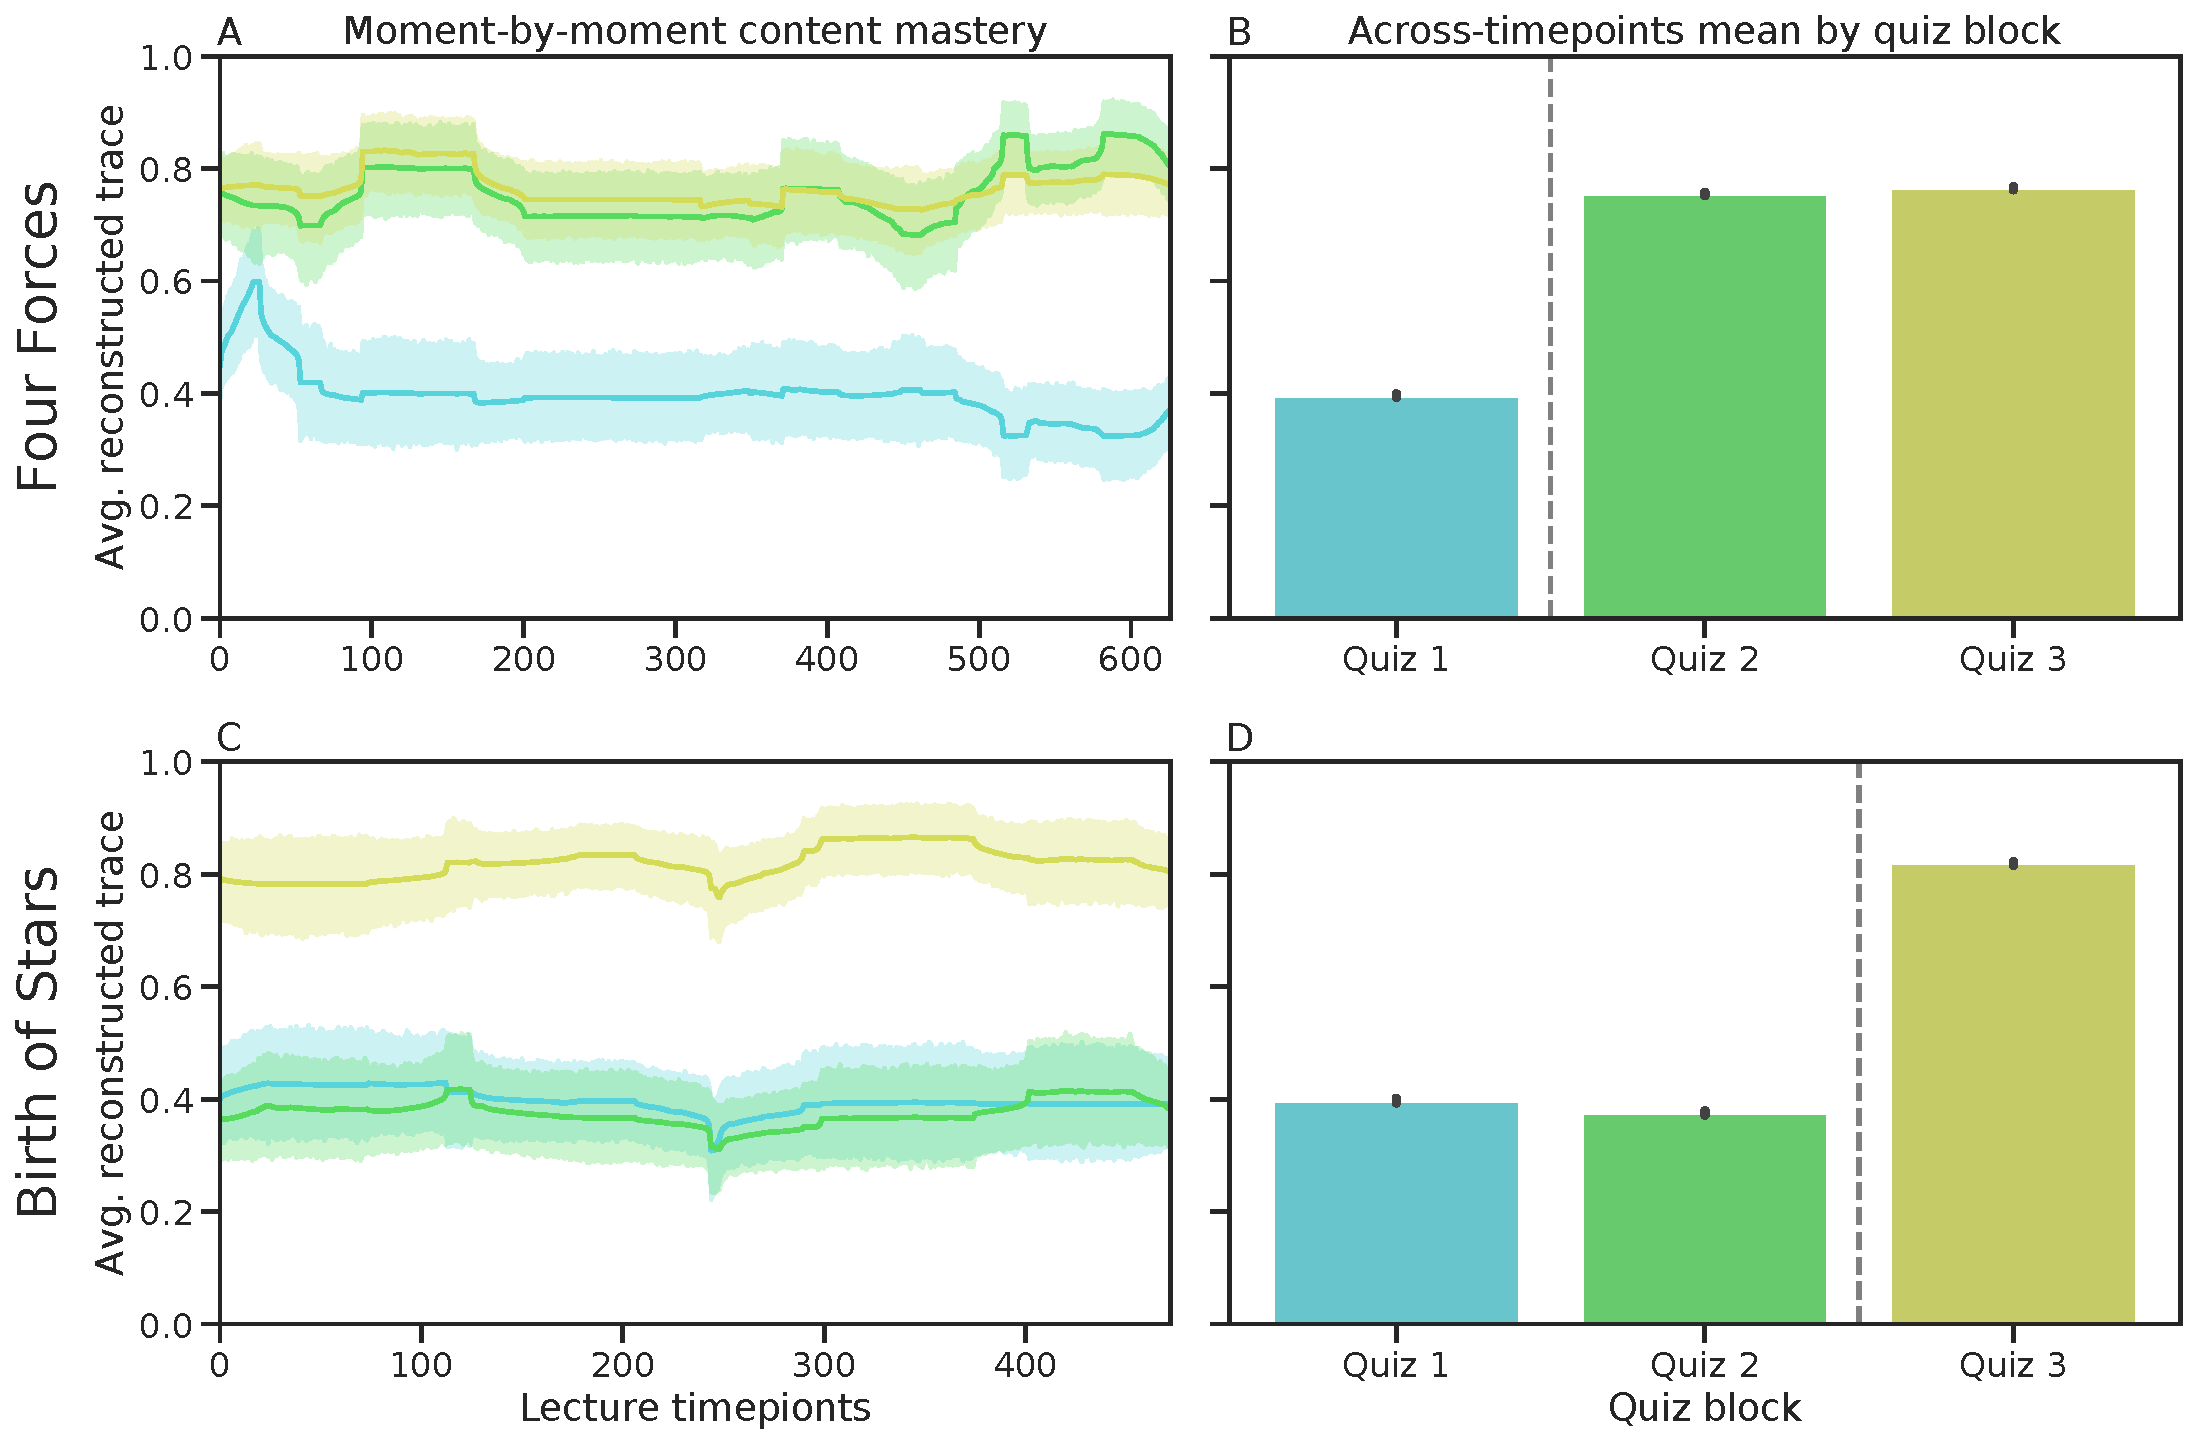
\includegraphics[width=0.7\textwidth]{figs/content-mastery}
    
    \caption{\textbf{Estimating moment-by-moment knowledge acquisition.}
    \textbf{A. Moment-by-moment knowledge about the \textit{Four Fundamental
    Forces}}. Each trace displays the weighted proportion of correctly answered
    questions about the content reflected in each moment of the lecture (see
    \textit{Estimating dynamic knowledge traces}), using responses from one
    quiz (color). The traces are averaged across participants. \textbf{B.
    Average estimated knowledge about the \textbf{Four Fundamental Forces}.}
    Each bar displays the across-timepoint average knowledge, estimated using
    the responses to one quiz's questions. \textbf{C. Moment-by-moment
    knowledge about the \textit{Birth of Stars}}. The panel is in the same
    format as Panel A, but here the knowledge estimates are for the
    moment-by-moment content of the \textit{Birth of Stars} lecture. \textbf{D.
    Average estimated knowledge about the \textit{Birth of Stars}.} The panel
    is in the same format as Panel B, but here the knowledge estimates are for
    the content of the \textit{Birth of Stars} lecture. All panels: error
    ribbons and error bars denote 95\% confidence intervals, estimated across
    participants.}
    
    \label{fig:knowledge-timeseries}
\end{figure}

\begin{figure}[tp]
    \centering
    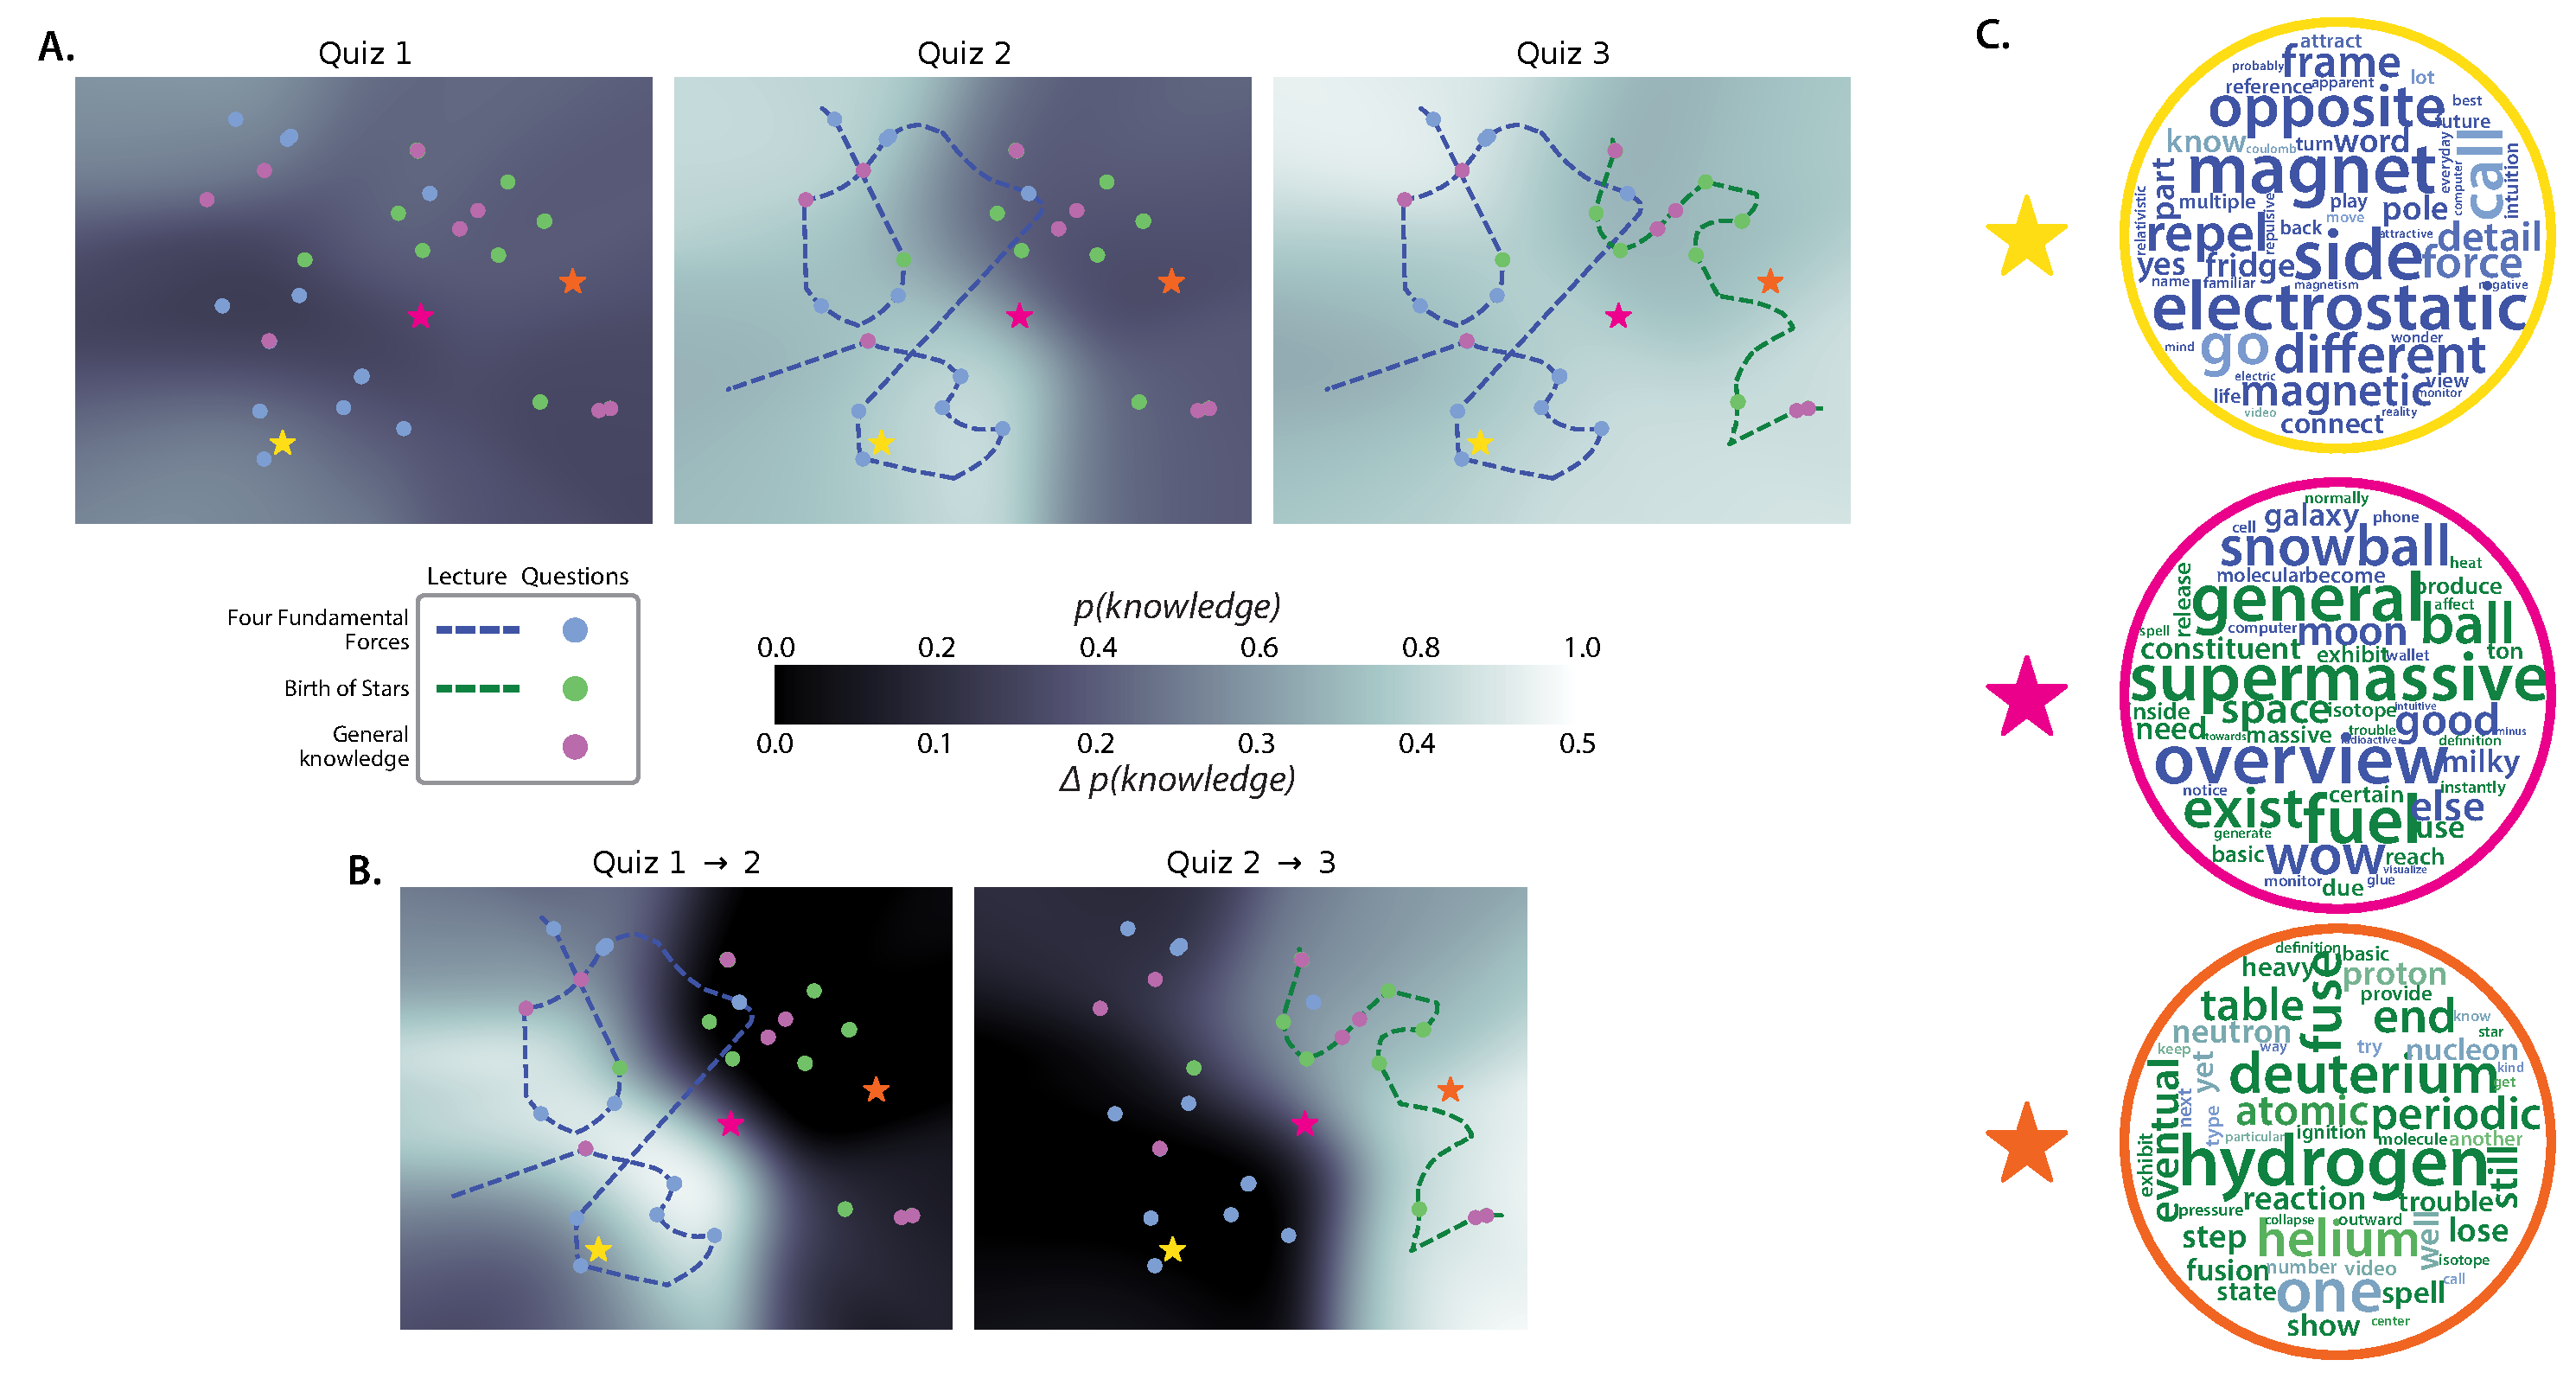
\includegraphics[width=\textwidth]{figs/knowledge_and_learning_maps}
    
    \caption{\textbf{Mapping out the geometry of knowledge and learning.}
    \textbf{A. Average ``knowledge maps'' estimated using each quiz.} Each map
    displays a 2D projection of the estimated knowledge about the content
    reflected by \textit{all} regions of topic space (see \textit{Creating
    knowledge and learning map visualizations}). The topic trajectories of each
    lecture and the coordinates of each question are indicated by dotted lines
    and dots. Each map reflects an average across all participants. For
    individual participants' maps, see
    Figures~\individualKnowledgeMapsA,~\individualKnowledgeMapsB,
    and~\individualKnowledgeMapsC. \textbf{B. Average ``learning maps''
    estiamted between each successive pair of quizzes.} The learning maps are
    in the same general format as the knowledge maps in Panel A, but each
    coordinate in the learning maps indicates the \textit{difference} between
    the corresponding coordinates in the indicated \textit{pair} of knowledge
    maps-- i.e., how much the estimated knowledge ``changed'' across the two
    quizzes. Each map reflects an average across all participants. For
    individual participants' maps, see
    Figures~\individualLearningMapsA~and~\individualLearningMapsB. \textbf{C.
    Word clouds for sampled points in topic space.} Each word cloud displays
    the relative weights of each word reflected by the blend of topics
    represented at the locations of the stars in the maps. The words' colors
    indicate how much each word is weighted on average across all timepoints'
    topic vectors in the \textit{Four Fundamental Forces} (blue) and
    \textit{Birth of Stars} (green) videos, respectively.}
    
    \label{fig:knowledge-maps}
    \end{figure}

\section*{Discussion}

\section*{Materials and methods}

\subsection*{Participants}

We enrolled a total of 50 Dartmouth undergraduate students in our study.
Participants received course credit for enrolling. We asked each participant to
fill out a demographic survey that included questions about their age, gender,
native spoken language, ethnicity, race, hearing, color vision, sleep, coffee
consumption, level of alertness, and several aspects of their educational
background and prior coursework.

Participants' ages ranged from 18 to 22 years (mean: 19.52 years;
standard deviation: 1.09 years). A total of 15 participants reported
their gender as male and 35 participants reported their gender as
female. A total of 49 participants reported their native language as
``English'' and 1 reported having another native language. A total of
47 participants reported their ethnicity as ``Not Hispanic or Latino''
and three reported their ethnicity as ``Hispanic or Latino.''
Participants reported their races as White (32 participants), Asian
(14 participants), Black or African American (5 participants),
American Indian or Alaska Native (1 participant), and Native Hawaiian or
Other Pacific Islander (1 participant). (Note that some participants
selected multiple recial categories.)

A total of 49 participants reporting having normal hearing and 1
participant reported having some hearing impairment. A total of 49
participants reported having normal color vision and 1 participant
reported being color blind.  Participants reported having had, on the
night prior to testing, 2 -- 4 hours of sleep (1 participant), 4 -- 6
hours of sleep (9 participants), 6 -- 8 hours of sleep (35
participants), or $8+$ hours of sleep (5 participants). They reported
having consumed, on the same day and leading up to their testing
session, 0 cups of coffee (38 participants), 1 cup of coffee (10
participants), 3 cups of coffee (1 participant), or $4+$ cups of
coffee (1 participant).

No participants reported that their focus was currently impaired
(e.g., by drugs or alcohol).  Participants reported their current
level of alertness, and we converted their responses to numerical
scores as follows: ``very sluggish'' (-2), ``a little sluggish'' (-1),
``neutral'' (0), ``fairly alert'' (1), and ``very alert'' (2). Across
all participants, a range of alertness levels were reported (range: -2
-- 1; mean: -0.10; standard deviation: 0.84).

Particpants reported their undergraduate major(s) as Social Sciences
(28 participants), Natural sciences (16), Professional (e.g., pre-med
or pre-law; 8 participants), Mathematics and engineering (7
participants), Humanities (4 participants), or Undecided (3
participants).  Note that some participants selected multiple
categories for their undergraduate major.  We also asked participants
about the courses they had taken.  In total, 46 participants reported
having taken at least one Khan academy course in the past or being
familiar with the Khan academy, and 4 reported not having taken any
Khan academy courses.  Of the participants who reported having watched
at least one Khan academy course, 1 participant declined to report the
number of courses they had watched; 7 participants reported having
watched 1--2 courses; 11 reported having watched 3--5 courses; 8
reported having watched 5--10 courses; and 19 reported having watched
10 or more courses.  We also asked participants about the specific
courses they had watched, categorized under different subject areas.
In the ``Mathematics'' area participants reported having watched
videos on AP Calculus AB (21 participants), Precalculus (17
participants), Algebra 2 (14 participants), AP Calculus BC (12
participants), Trigonometry (11 participants), Algebra 1 (10
participants), Geometry (8 participants), Pre-algebra (7
participants), Multivariable Calculus (5 participants), Differential
Equations (5 participants, Statistics and Probability (4
participants), AP Statistics (2 participants), Linear Algebra (2
participants), Early Math (1 participant), Arithmetic (1 participant),
and other videos not listed in our survey (6 participants).  In the ``Science and engineering''
area participants reported having watched videos on Chemistry, AP
Chemistry, or Organic Chemstry (21
participants); Physics, AP Physics I, or AP Physics II (15 participants); Biology, AP
Biology; or High school Biology (15 participants); Health and Medicine
(1 participant); or other videos not listed in our survey (20 participants).  We also asked
participants if they had specifically seen the videos used in our
experiment.  When we asked about the \textit{Four Fundamental Forces}
video, 45 participants reported not having watched it before, 1
participant reported that they were not sure if they had watched it
before, and 4 participants declined to respond.  When we asked about
the \textit{Birth of Stars} video, 46 participants reported not having
watched it before and 4 participants declined to respond.  When we
asked participants about non-Khan academy online courses, they
reported having watched or taken courses on Mathematics (15
participants), Science and engineering (11 participants), Test
preparation (9 participants), Economics and finance (3 participants),
Arts and humanities (2 participants), Computing (2 participants), and
other categories not listed in our survey (18 participants).  Finally,
we asked participants about in-person courses they had taken in
different subject areas.  They reported taking courses in Mathematics
(39 participants), Science and engineering (38 participants), Arts and
humanities (35 participants), Test preparation (27 participants),
Economics and finance (26 participants), Computing (15 participants),
College and careers (7 participants), or other courses not listed in
our survey (6 participants).


\subsection*{Experiment}

We hand-selected two roughly 10-minute course videos from the Khan Academy
platform: \textit{The Four Fundamental Forces} (an introduction to gravity,
electromagnetism, the weak nuclear force, and the strong nuclear force;
duration: 10 minutes and 29 seconds) and \textit{Birth of Stars} (an
introduction to how stars are formed; duration: 7 minutes and 57 seconds). We
hand-wrote 39 multiple choice questions: 15 about the conceptual content of
\textit{The Four Fundamental Forces}, another 15 about the conceptual content
of \textit{Birth of Stars}, and 9 other questions that tested for general
conceptual knowledge about basic physics (covering material that was not
presented in either video). The full set of questions may be found in
Table~\questions.



Participants began the main experiment by answering a battery of 13 randomly
selected questions (chosen from the full set of 39). Then they watched the
\textit{The Four Fundamental Forces} video. Next, they answered a second set of
13 questions (chosen at random from the remaining 26 questions). Fourth,
participants watch the \textit{Birth of Stars} video, and finally they answered
the remaining 13 questions. Our experimental procedure is diagramed in
Figure~\ref{fig:experiment}. We used the experiment to develop and test our
computational framework for estimating knowledge and learning maps.

\subsection*{Analysis}

\subsubsection*{Constructing text embeddings of multiple videos and questions}

We extended an approach developed by~\citep{HeusEtal21} to construct text
embeddings for each moment of each lecture, and of each question in our pool.
Briefly, our approach uses a topic model~\citep{BleiEtal03}, trained on a set
of documents, to discover a set of $k$ ``topics'' or ``themes.'' Formally, each
topic is defined as a set of weights over each word in the model's vocabulary
(i.e., the union of all unique words, across all documents, excluding ``stop
words.''). Conceptually, each topic is intended to give larger weights to set
of words that appear conceptually related or that tend to co-occur in the same
documents. After fitting a topic model, each document in the training set, or
any \textit{new} document that contains at least some of the words in the
model's vocabulary, may be represented as a $k$-dimensional vector describing
how much the document (most probably) reflects each topic. (Unless, otherwise
noted, we used $k = 15$ topics.)

\begin{figure}[tp]
\centering
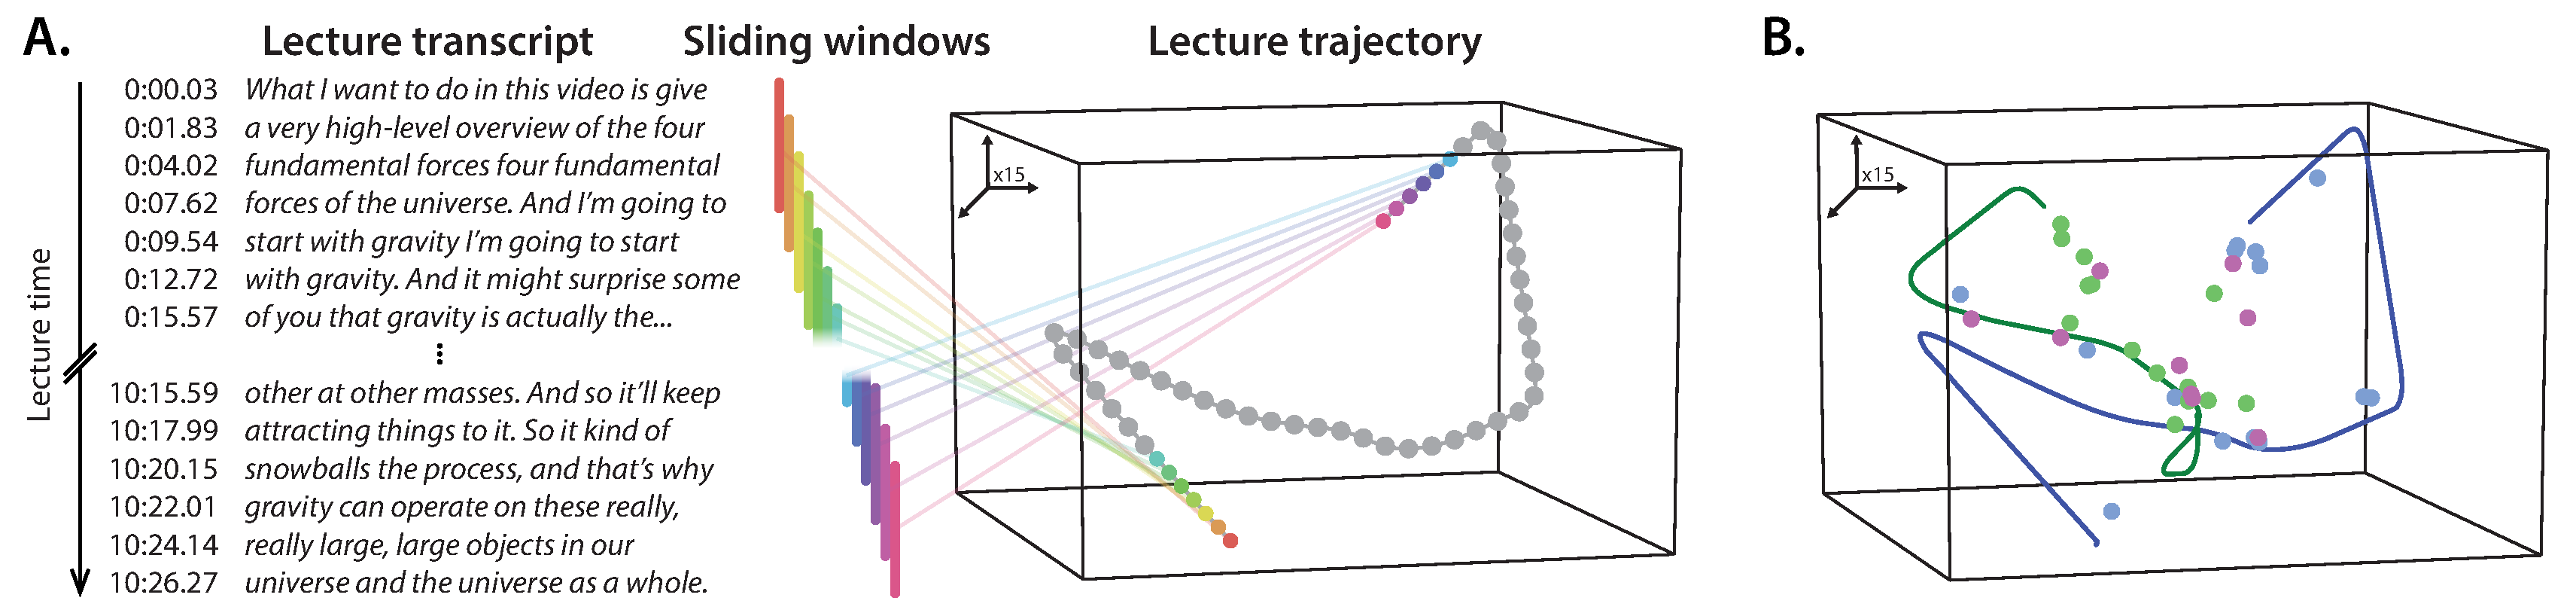
\includegraphics[width=\textwidth]{figs/sliding_windows}

\caption{\textbf{Constructing video content \textit{trajectories}. \textbf{A.
Building a document pool from sliding windows of text.} We decompose each
video's transcript into a series of overlapping sliding windows. The set of
transcript snippets (across all windows) may be treated as a set of
``documents'' for training a text embedding model. After training a text
embedding model using the two videos' sliding windows, along with the text from
each question in our pool (Tab.~\questions), } we construct ``trajectories''
through text embedding space by joining the embedding coordinates of successive
sliding windows from each video. \textbf{B. Embedding multiple videos and
questions.} Applying the same text embedding approach to each video, along with
the text of each question, results in one trajectory per video and one
embedding coordinate (dot) per question (blue: Four Fundamental Forces; green:
Birth of Stars; pink: general physics knowledge). Here we have projected the
15-dimensional embeddings into a 3D space using Uniform Manifold Approximation
and Projection~\citep[UMAP;][]{McInEtal18a}.}

\label{fig:sliding-windows}
\end{figure}

As illustrated in Figure~\ref{fig:sliding-windows}A, we start by building up a
corpus of documents using overlapping sliding windows that span each video's
transcript. Khan Academy videos are hosted on the YouTube platform, and all
YouTube videos are run through Google's speech-to-text API~\citep{HalpEtal16}
to derive a timestamped transcript of any detected speech in the video. The
resulting transcripts contain one timestamped row per line, and each line
generally corresponds to a few seconds of spoken content from the video. We
defined a sliding window length of (up to) $w = 30$ transcript lines, and we
assigned each window a timestamp according to the midpoint between its first
and last lines' timestamps. These sliding windows ramped up and down in length
at the very beginning and end of the transcript, respectively. In other words,
the first sliding window covered only the first line from the transcript; the
second sliding window covered the first two lines; and so on. This insured that
each line of the transcript appeared in the same number ($w$) of sliding
windows. We treated the text from each sliding window as a single ``document,''
and we combined these documents across the two videos' windows to create a single
training corpus for the topic model.  The top words from each of the 15 discovered
topics may be found in Table~\topics.

After fitting a topic model to each videos' transcripts, we could use the
trained model to transform arbitrary (potentially new) documents into
$k$-dimensional topic vectors. A convenient property of these topic vectors is
that documents that reflect similar blends of topics (i.e., documents that
reflect similar themes, according to the model) will yield similar (in terms of
Euclidean distance, correlation, etc.) topic vectors. In general, the
similarity between different documents' topic vectors may be used to
characterize the similarity in content between the documents.

We transformed each sliding window's text into a topic vector, and then used
linear interpolation (independently for each topic dimension) to resample the
resulting timeseries to once per second. This yielded a single topic vector for
each second of each video. We also used the fitted model to obtain topic
vectors for each question in our pool (Tab.~\questions). Taken together, we
obtained a \textit{trajectory} for each video, describing its path through
topic space, and a single coordinate for each question
(Fig.~\ref{fig:sliding-windows}B). Embedding both videos and all of the
questions using a common model enables us to compare the content from different
moments of videos, compare the content across videos, and estimate potential
associations between specific questions and specific moments of video.


\subsubsection*{Estimating dynamic knowledge traces}

We used the following equation to estimate each participant's knowledge about
timepoint $t$ of a given lecture, $\hat{k}(t)$:
\begin{equation} 
    \hat{k}(t) = \frac{\sum_{i \in \mathrm{correct}}\mathrm{ncorr}(t, i)}{\sum_{j = 1}^N \mathrm{ncorr}(t, j)},
    \label{eqn:prop}
\end{equation}
where 

\begin{equation} 
    \mathrm{ncorr}(x, y) = \frac{\mathrm{corr}(x, y) - \mathrm{mincorr}}{\mathrm{maxcorr} - \mathrm{mincorr}},
\end{equation} 
and where $\mathrm{mincorr}$ and $\mathrm{maxcorr}$ are the minimum and maximum
correlations between any lecture timepoint and question, taken over all
timepoints and questions across both lectures and all three question sets.

Intuitively, $\mathrm{ncorr}(x, y)$ is the correlation between two topic
vectors (e.g., the topic vector from one timepoint in a lecture, $x$, and the
topic vector for one question, $y$), normalized by the minimum and maximum
correlations (across all timepoints and questions) to range between 0 and 1,
inclusive. Equation~\ref{eqn:prop} then computes the weighted average
proportion of correctly answered questions about the content presented at
timepoint $t$, where the weights are given by the normalized correlations
between timepoint $t$'s topic vector and the topic vectors for each question.
The normalization step (i.e., using $\mathrm{ncorr}$ instead of the raw
correlations) insures that every question (except the least-relevant question)
contributes some non-zero amount to the knowledge estimate.

\subsubsection*{Estimating held-out conceptual knowledge}

\subsubsection*{Creating knowledge and learning map visualizations}

An important feature of our approach is that, given a trained text embedding
model and participants' quiz performance on each question, we can estimate
their knowledge about \textit{any} content expressable by the embedding model--
not solely the content explicitly probed by the quiz questions. To visualize
these estimates
(Figs.~\ref{fig:knowledge-maps},~\individualKnowledgeMapsA,~\individualKnowledgeMapsB,~\individualKnowledgeMapsC,~\individualLearningMapsA,
and~\individualLearningMapsB), we used UMAP~\citep{McInEtal18a} to define a 2D
projection of the text embedding space. Sampling the original 100-dimensional
space at high resolution to obtain an adequate set of topic vectors spanning
the embedding space would be computationally intractable. However, sampling a
2D grid is much more feasible. We defined a rectangle enclosing the 2D
projections of the lectures' and quizzes' embeddings, and we sampled points
from a regular $100 \times 100$ grid of coordinates that evenly tiled the
enclosing rectangle. We sought to estimate participants' knoweldge (and
learning-- i.e., changes in knowledge) at each of the resulting 10000
coordinates.

To generate our estimates, we placed a set of 39 radial basis functions (RBFs)
throughout the embedding space, centered on the 2D projections for each
question (i.e., we included one RBF for each question). At coordinate $x$, the
value of an RBF centered on a question's coordinate $\mu$, is given by:
\begin{equation}
    \mathrm{RBF}(x, \mu, \lambda) = \exp\left\{-\frac{||x - \mu||^2}{\lambda}\right\}.
    \label{eqn:rbf}
\end{equation}
The $\lambda$ term in the RBF equation controls the ``smoothness'' of the
function, where larger values of $\lambda$ result in smoother maps. In our
implementation we used $\lambda = 50$.  Next, we estimated the ``knowledge''
at each coordinate, $x$, using:
\begin{equation}
    \hat{k}(x) = \frac{\sum_{i \in \mathrm{correct}} \mathrm{RBF}(x, q_i, \lambda)}{\sum_{j = 1}^N \mathrm{RBF}(x, q_j, \lambda)}.
    \label{eqn:rbf-knowledge}
\end{equation}
Intuitively, Equation~\ref{eqn:rbf-knowledge} computes the weighted proportion of
correctly answered questions, where the weights are given by how nearby (in the 2D space)
each question is to the $x$.  We also defined \textit{learning maps} as the coordinate-by-coordinate
differences between any pair of knowledge maps.  Intuitively, learning maps reflect the \textit{change}
in knowledge across two maps.


\bibliographystyle{apa}
\bibliography{CDL-bibliography/cdl}
\end{document}
